\chapter{Sign language animation}

In this chapter, we will review the state of the art about signing language 
animation using 3D avatars...

\section{Sign language animation}

Sign language avatars promise to become an indispensable and inclusive reservoir of natural language communication for the signing deaf community. However, developing top-tier avatars demands substantial commitments in terms of time and financial resources. Crafting these high-quality avatars poses a formidable engineering challenge \cite{quandt2020teaching}.


Specific requirements must be satisfied within the avatar file to animate any avatar. These prerequisites include a mesh, a skeleton, a texture, and a collection of morph targets if facial animation is necessary. The mesh 
serves as the outward visual representation of the avatar and, in conjunction with 
the texture, defines the avatar's optical characteristics. The skeleton, though 
imperceptible in the software, consists of interconnected bones, each linked to the 
vertices within the mesh. Consequently, altering the rotation of any bone within 
the skeleton leads to corresponding movements in the mesh vertices connected to it. 
The morph targets, also known as blend shapes, play a crucial role in deforming the 
static mesh. They modify the area around the mouth and jaw for 
speech synchronization and to manipulate the cheeks, eyelids, eyebrows, and 
forehead to convey various facial expressions \cite{jennings2010requirements}.

JASigning is a synthetic animation system for deaf signing, written in Java, that 
has been developed at UEA, taking as input avatar-independent Gestural SiGML 
(Signing Gesture Markup Language) \parencite{elliott2004overview, 
elliott2008linguistic} and producing output motion data for any avatar. SiGML is an 
XML form of HamNoSys (Hamburg Notation System) (Prillwitz et al., 1989; Hanke, 
2004). Animgen uses that (Kennaway, Glauert, Zwitserlood, 2007) To generate 
Signing animation. To achieve this, JASigning requires additional information that 
cannot be obtained from the standard information above and must be provided in 
separate files \cite{jennings2010requirements}.

For the JASigning software, four avatar definition files effectively define each. 
ARP signing avatar. The first of these contains binary data, the other three are
XML: Main Avatar Definition, ASD  Avatar Standard Description,  Animgen Configuration Data, Nonmanuals.

\textbf{Main Avatar Definition} 

\textbf{Vertex list}

A list of vertices representing the mesh defining the avatar's shape, with texture coordinates and vertex normals for each.

\textbf{Texture map}
Defines the appearance of the avatar.

\textbf{skeleton}
The skeleton structure fits within the mesh. It must include all bone names used by 
Animgen.

\textbf{Mesh-to-Skeleton Attachment Data}

This data is a list of links between vertices in the mesh and
the bone(s) that will animate them, with a weight for the influence
of each bone. A maximum of 4 links per vertex is
permitted, with a preferred maximum of 3. The weights of
all links to a vertex must sum to 1.0. This follows standard
industry practice for this data type, as more than four links
to a vertex make weight calculations very complex.\\


\section{Ways to generate an Avatar}

Generating signing avatars through motion capture recordings of native signers can yield significantly more naturalistic results than avatars constructed solely from computer-generated models. Nevertheless, it's essential to acknowledge that the creation of motion-captured avatars demands a considerably higher level of manual labor and presents limitations in automation and the ability to iteratively generate new content compared to avatars generated using computational algorithms \parencite{quandt2020teaching}.


\section{Sign language synthesis}

Sign and utterance synthesis are fundamentally distinct processes 
within sign language technology. Sign synthesis involves the 
creation of skeletal animations for individual signs, focusing on 
isolated linguistic units. In contrast, utterance synthesis 
encompasses the animation of entire sign language sentences, 
necessitating a deeper understanding of sign language linguistics 
and involving distinct mechanisms compared to generating isolated 
signs. To achieve coherent sign language communication, it is 
imperative to consider sign language grammar, ensuring that the 
generated utterances maintain consistency and fidelity to the 
linguistic rules and structure of the specific sign language in 
question \parencite{naert2020survey}.

\subsection{Isolated sign synthesis}

There are two distinct linguistic approaches to animating signing avatars in sign language (SL). The first parametric approach operates at a phonological level and primarily synthesizes isolated signs. This approach focuses on the specific phonological parameters of signs. The second approach concentrates on the sign inflection mechanisms, addressing the more variable and fluid aspects of sign language at a linguistic level. This latter approach is especially relevant during the synthesis of utterances, where the context and fluidity of speech play a significant role \parencite{naert2020survey}.

\subsection{The parametric approach}


To create signs, sign languages use multiple components, such as 
hand configuration, placement, movement, and orientation 
\parencite{naert2020survey}. Unlike vocal languages that construct 
words through a linear sequence of phonemes, sign languages operate 
on both simultaneous and sequential levels. This unique feature of 
utilizing various elements simultaneously is why sign languages are 
described as multilinear. This multilinear nature allows for a rich 
and complex form of communication 
\parencite{sallandre2007simultaneity}.\\

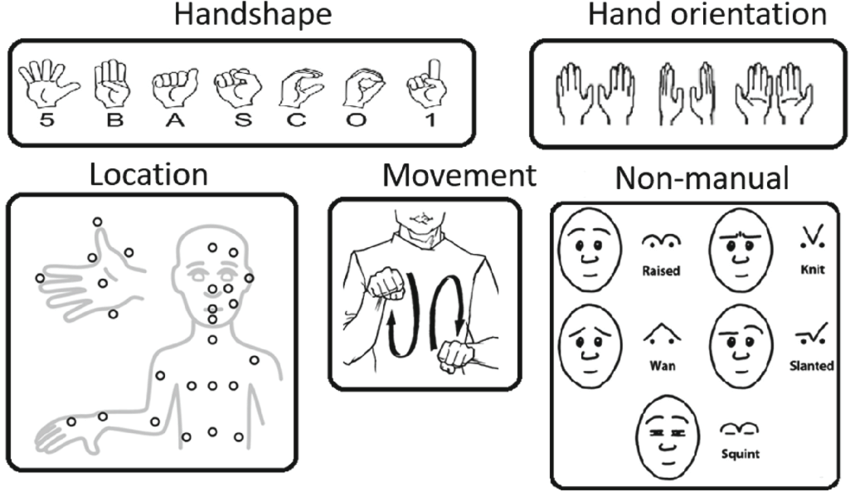
\includegraphics[width=\textwidth]{figures/signcomponents.png}
\captionof{figure}{Extract from \textcite{signlanguagerecogn} Five components of signs in sign language }


The parametric approach to sign language involves constructing signs 
by setting specific values for various phonological parameters and 
combining these into a single virtual character. The combination of 
its parameters uniquely defines each sign. This method focuses on 
creating posters with stable characteristics, ensuring consistency and 
clarity in the language \parencite{naert2020survey}.




\section{Representations of signs}

 For isolated signs, typically synthesized using a parametric approach, this representation needs to emphasize both the structure of the sign and the values of its phonological elements during its production. The spatiotemporal nature of sign languages, which involves space and time dimensions, makes the exhaustive representation of signs challenging. This complexity requires collaboration between experts in linguistics and computer animation. The goal is to accurately capture sign language's dynamic and multifaceted nature, encompassing the physical movements and the linguistic principles underlying them \parencite{naert2020survey}.

 \textcite{naert2020survey} mention three ways of signs representation used in the study of signs: visual representations, gloss representation, parametric notation, and writing systems. In Table 1, there is a comparison of the different sign representations. 

 \subsection{Visual representations}

Visual representations convey ideas, information, or data through a visual format. In this case, to represent signs. According to \textcite{naert2020survey}, the process involves representing signs on a 2D canvas, aiming to be as accurate as possible to the symbol used in sign language since signs involve movements in three-dimensional space and time. Drawings and video recordings are two typical ways of visual sign representations.\\

\subsubsection{Drawings}

Drawings represent the signs on a 2-D canvas by being faithful to the actual sign.
Signs are motions specified both in the 3D space and in time: in a drawing, using arrows and different types of contour (e.g., dotted line or fine line) allows for a partial representation of those dimensions on a 2D paper (See fig. ). However, this schematic representation depends on the user's interpretation and the artist's skill. Drawings are an ambiguous representation that often needs to be clarified with annotations \parencite{naert2020survey}.\\

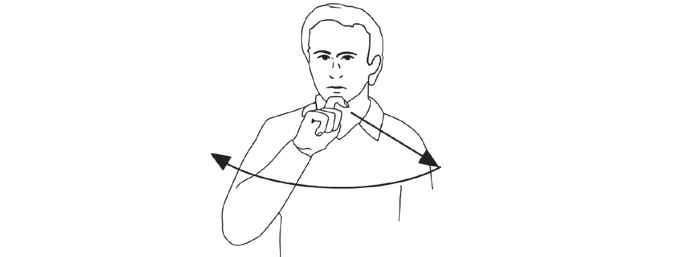
\includegraphics[width=\textwidth]{figures/drawing-isl.jpg}
\captionof{figure}{Extract from from McDonnell (1996) Drawing}



\subsubsection{Videos}

Videos, once produced, are static, meaning they cannot be altered or modified post-production. Additionally, the inability to anonymize individuals in videos is a crucial concern in sign language representation, as the face plays an integral role in meaning through expressions and mouth shapes. The facial component of sign language is essential for complete communication \parencite{kipp2011assessing}. Also, videos are good for capturing the dynamics of sign language. Still, they have disadvantages, including flattening the depth of information, imposing a specific viewpoint on the viewer, and omitting spatial details. Like drawings, their format and limitations render them unsuitable for representing signs in an automated animation engine, which requires a more adaptable and detailed form of representation \parencite{naert2020survey}.

\subsection{Parametric Notation}

\subsubsection{Stokoe}

Stokoe identified three key linguistic elements in his research: the configuration of the hand, hand placement, and hand motion (see section 2.2 for details). Stokoe's notation system represents American Sign Language (ASL) signs. In this system, the sign location is termed 'tabula' or TAB, the configuration of the hand is known as 'designator' or DEZ, and the hand motion is referred to as 'signature' or SIG. These components are each defined using a specific set of symbols \parencite{stokoe2005sign}.

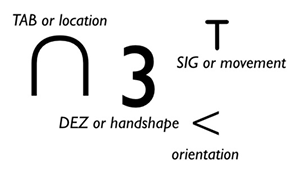
\includegraphics[width=\textwidth]{figures/stokoe-notation.PNG}
\captionof{figure}{Extract from Julie A. Hochgesang for Linguistics 101 at Gallaudet University, 2007}

\subsubsection{HamNoSys}

The Hamburg Notation System for Sign Languages (HamNoSys) is based on the Stokoe notation system, developed by Stokoe in 1960, which was an alphabetic system for describing the sublexical parameters - location, hand configuration (primarily handshape), and movement - of American Sign Language signs. HamNoSys extends this approach, providing an alphabetic system for representing signs, primarily at a phonetic level \parencite{prillwitz1989hamnosys}. 

The parameters of a sign are documented in a specific sequence: first, the symmetry operator, followed by nonmanual components, then hand shape, hand position, location, and finally, movement \parencite{kaur2014hamnosys}.




\subsubsection{SLPA}

The Sign Language Phonetic Annotation (SLPA) framework uses the Posture-Detention-Transition-Shift (PDTS) classification to analyze sign language. It categorizes segments or timing units based on two-timing characteristics: the static/dynamic nature and the transient/deliberate quality of motion. Static segments maintain certain sign language components (like hand configuration, orientation, placement, and non-manual features) unchanged for a period, while dynamic segments mark a transition between static ones \parencite{naert2020survey}. The transient/deliberate quality affects the duration of these segments. SLPA identifies four types of timing units: Posture (static and transient), Detention (static and deliberate), Transform (dynamic and transient), and Shift (dynamic and deliberate). To transcribe a sign, SLPA uses a table format with timing units in columns and articulatory components in rows \parencite{johnson2011segmental}.

\subsubsection{SignWriting}

The SIGNWRITING system is a method for documenting deaf sign languages using a collection of intuitive, graphical-schematic symbols. These symbols and straightforward rules for their combination enable the representation of signs. Due to its graphical nature, SIGNWRITING requires properly encoding its symbols for digital applications. This encoding is essential for storing and processing sign language documents on computers and integrating written sign languages into interactive elements of computer program interfaces \parencite{da2003signwriting}.

\subsection{Scripting language}


\subsubsection{SWML}

The SIGNWRITING MARKUP LANGUAGE (SWML) is an XML-based language designed to facilitate interoperability among systems that process sign languages using SignWriting. SWML can represent SIGNWRITING texts and dictionaries created by programs like SIGNWRITER and SW-EDIT \parencite{da2003signwriting}.

A signbox, which represents a sign, contains the same information as its SignWriting transcription. However, it shares SignWriting's limitations, including ambiguities in hand placement and time management \parencite{naert2020survey}.


\subsubsection{SiGML}

SiGML (Signing Gesture Markup Language) is an XML dialect created for detailing sign language sequences for depiction by a virtual human (VH) signer or avatar. It is closely modeled on the HamNoSys notation, originally developed for transcribing human signing. Like HamNoSys, SiGML describes sign language at the phonetic level. Its scope and role are focused on this aspect, though it differs in other respects \parencite{glauert2011extending}.

SiGML, like HamNoSys, breaks down the description of a sign into a structured format. In its manual part, it represents features like hand shape, orientation, location, and movement. This movement category encompasses not only changes in location but also alterations in hand shape and orientation \parencite{glauert2011extending}.

Developed under the European projects ViSiCAST and eSIGN, which aim to enhance Deaf access to information \parencite{kennaway2003experience}, this language was created to animate virtual signers. Consequently, it allows for more detailed specifications in aspects like timing and precise orientations in SiGML, features that are not as explicitly detailed in HamNoSys \parencite{naert2020survey}. The PDTS classification, developed by Johnson and Liddell, was integrated into an extended version of SiGML \parencite{glauert2011extending}, enhancing the language with explicit timing control, synchronization of elementary motions, and detailed direction specifications in various contexts. This addition positions it as one of the most advanced sign language specifications available for sign language synthesis \parencite{naert2020survey}.

\subsubsection{QualGest}

\textcite{lebourque1999high} defined QualGest, a
high-level specification language dedicated to French Sign Language (LSF) that takes into
account the four manual parameters (hand configuration, place-
ment, motion and orientation), called gestems.

QualGest (Qualitative Gestures specification) system is a \textcite{lebourque1999high} proposal that includes a spatial representation around the signer and a set of movement primitives, hand configurations, and orientations. These elements are combined to describe a gesture, which comprises components that can occur sequentially or in parallel. At a more detailed level, various sign parameters, such as orientation, configuration, movement, and location, are combined simultaneously. Moreover, many signs consist of multiple sub-gestures that occur sequentially. Furthermore, there is a need for a preparatory phase in gesturing, where a gesture starts with a specific hand and arm configuration. This preparation phase and the gesture itself occur in sequence. An imperative language is proposed to describe the composition of gestures hierarchically. Initially, movement, configuration, and orientation primitives are sequentially assembled to form elementary movements. These are then combined sequentially or in parallel to create a complete gesture. Finally, a gestural sentence is defined as a succession of these gestures \parencite{lebourque1999high}.

\subsubsection{Losson}

According to \textcite{naert2020survey} Losson's approach to sign language description segments signs into basic gestures named shifts, characterized by the hand's initial and final configurations, orientation, placement, and movement type. Hand movements are defined using basic displacement forms such as straight lines, arcs, or circles, along with the intended hand destination and, for arcs and circles, the plane's equation in which the movement occurs. Additional movements, contact areas, or modifiers can enhance these basic forms. In defining hand configurations, the thumb's behavior is considered separately from the other fingers, akin to the hand configuration coding in SLPA. Features such as movement repetition, hand synchronicity, symmetry or asymmetry, and the relative positioning of the hands are also specified. Additionally, Losson's model incorporates a parametric computer language for detailing sign inflection mechanisms, including size and shape details and spatial referencing.

\subsubsection{Zebedee}

Zebedee is a sign language specification language defined by geometrical concepts. Instead of traditional parameters like hand configuration, orientation, and placement, it uses geometric constraints on points, vectors, or surfaces \parencite{naert2020survey}. The Zebedee model categorizes signs into two temporal units, aligning with Liddell and Johnson's Movement/Hold model: key postures, where motion parameters stabilize, and transitions between these postures. A notable advantage of this model is its ability to represent sign inflections through modifications in the geometric constraints that describe each sign. Zebedee effectively captures both the temporal and spatial aspects of sign languages, and its geometric basis emphasizes the structural elements of signs \parencite{filhol2008modele}.

\subsubsection{EMBRScript}

\textcite{heloir2010real} introduced EMBR1 (Embodied Agents Behavior Realizer) and its accompanying control language, EMBRScript, enabling users to focus on intent and behavior planning. Users can input high-level behavior descriptions in the Behavior Markup Language (BML), which EMBR1 then converts into animations. An intermediate 'animation layer' is also proposed, providing access to animation parameters closely related to motion generation mechanisms, like spatiotemporal constraints. This layer allows direct interaction with the realizer's functionalities while simplifying the complexities of its implementation.

The animation layer offers a language for users to specify detailed output animations without needing extensive knowledge in computer animation. Additionally, the concepts of this layer serve as foundational elements for formally describing behaviors in BML.

The framework also includes methods to control motion quality, encompassing spatial and temporal extents, power, and fluidity. They introduce new formulations for realizing these motion qualities in individual motions, based on the concept of a nucleus, which encompasses both the stroke and the independent hold of a gesture.


\begin{landscape}
 \begin{table}[h]
 \fontsize{9pt}{9pt}\selectfont
     \centering
     \begin{tabular}
     {p{3cm} p{2.5cm} p{1.5cm} p{2.8cm} p{1.5cm} p{1.5cm} p{2.5cm}}
     \toprule
          Category &  Name&  Fidelity&  Temporal aspects, syncronization&  NMF&  Flexibility& Understandable by a computer\\  
    \midrule
    Visual representation &  Drawings & \cellcolor{lime} \checkmark &  \cellcolor{red} \XSolidBrush & \cellcolor{lime}  & \cellcolor{red}  & \cellcolor{red} \\ 
          & Video recordings & \cellcolor{green} \checkmark \checkmark  & \cellcolor{green} \checkmark \checkmark  & \cellcolor{green} \checkmark \checkmark & \cellcolor{red} \XSolidBrush  & \cellcolor{red} \XSolidBrush\\ 
     Parametric Notation     & Stokoe & \cellcolor{yellow} (\checkmark)  & \cellcolor{red} \XSolidBrush  & \cellcolor{red} \XSolidBrush &  \cellcolor{yellow} (\checkmark)  & \cellcolor{red} \XSolidBrush  \\ 
          & HamNoSys  & \cellcolor{lime} \checkmark  & \cellcolor{yellow} (\checkmark)  & \cellcolor{yellow} (\checkmark) & \cellcolor{yellow} (\checkmark) & \cellcolor{yellow} (\checkmark) \\ 
          & SLPA & \cellcolor{lime} \checkmark & \cellcolor{lime} \checkmark & \cellcolor{red} \XSolidBrush & \cellcolor{yellow} (\checkmark) & \cellcolor{yellow} (\checkmark) \\ 
          & SignWriting & \cellcolor{lime} \checkmark & \cellcolor{yellow} (\checkmark)  & \cellcolor{yellow} (\checkmark) & \cellcolor{yellow} (\checkmark)  & \cellcolor{red} \XSolidBrush \\  
     Scripting Language     & SiGML & \cellcolor{lime} \checkmark & \cellcolor{lime} \checkmark  & \cellcolor{yellow} (\checkmark)  & \cellcolor{yellow} (\checkmark) &  \cellcolor{green} \checkmark \checkmark\\  
          & QualGest & \cellcolor{lime} \checkmark & \cellcolor{lime} \checkmark & \cellcolor{red} \XSolidBrush & \cellcolor{lime} \checkmark & \cellcolor{green} \checkmark \checkmark \\ 
          & Losson &  \cellcolor{lime} \checkmark & \cellcolor{lime} \checkmark &  \cellcolor{yellow} (\checkmark) & \cellcolor{lime} \checkmark & \cellcolor{green} \checkmark \checkmark \\  
          & Zebedee & \cellcolor{lime} \checkmark &  \cellcolor{lime} \checkmark & \cellcolor{red} \XSolidBrush & \cellcolor{green} \checkmark \checkmark & \cellcolor{green} \checkmark \checkmark \\ 
          & EMBRScript & \cellcolor{lime} \checkmark & \cellcolor{lime} \checkmark  &  \cellcolor{yellow} (\checkmark) & \cellcolor{lime} \checkmark  & \cellcolor{green} \checkmark \checkmark \\ 
    \bottomrule
     \end{tabular}
    
     \caption{Taken from \parencite{naert2020survey} Comparison of the sign representation}
     \label{tab:visualrepresentations}
 \end{table}
\end{landscape}

Fidelity : absence of ambiguity, fidelity to the original movement, precise description of the sign, preservation of the intent of the signer. Temporal aspects, synchronization : the dynamics of the movement is specified, the synchronization between the different channels is managed. Non manual features : the status of non-manual components (facial expressions, gaze, etc.) is specified/visible. Flexibility : the ease with which the representation of a sign is modified to take into account the context of the sentence. A purely visual representation will make the transformation fastidious while some linguistic representations are highly flexible. Understandable by a computer : it can be reused as it is at the input of an automatic synthesis engine. 


\subsubsection{Behavioural Markup Language BML}

BML, or Behavior Markup Language, is an XML-based scripting language designed for seamless integration into larger XML messages or documents. To incorporate BML functionality, a simple initiation involves encapsulating a set of behaviors within a designated <bml> block (see fig. 4.4), thereby instructing an animated agent on the actions it should manifest \parencite{vilhjalmsson2007behavior}.

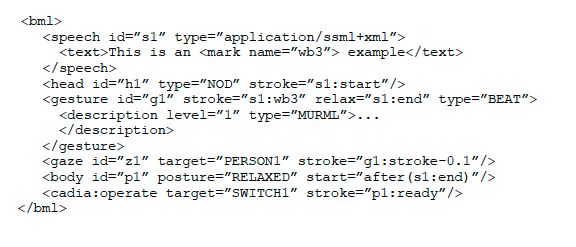
\includegraphics[width=\textwidth]{figures/bml-example.png}
\captionof{figure}{Extracted from \parencite{vilhjalmsson2007behavior} section 2, BML block example}

This specialized block serves as a coordinating mechanism for speech, gesture, gaze, head and body movements, consolidating them by including corresponding behavior elements within a singular encompassing element. Additional <bml> behavior elements encompass torso, face, legs, lips, and a wait behavior. Each behavioral directive undergoes a structured organization into six distinct animation phases, demarcated by sync-points that bear the names of associated motion transitions \parencite{vilhjalmsson2007behavior}.

The synchronization process involves seven key sync-points: start, ready, stroke-start, stroke, stroke-end, relax, and end. Achieving synchrony between behaviors is facilitated by aligning the sync-points of different behaviors, thereby orchestrating a seamless coordination of actions at specific points in time. In the aforementioned example, the head nod's most exertive phase, the stroke, precisely coincides with the designated sync-point, demonstrating the intricacies of temporal alignment within the BML framework \parencite{vilhjalmsson2007behavior}.

A recent augmentation to BML involves the incorporation of "levels of description," a feature designed to offer a more intricate portrayal of behaviors beyond the capabilities of the fundamental BML tags and attributes (see fig. 4.5). Specifically, the integration of a MURML type description for the gesture alongside the essential BML gesture element \parencite{vilhjalmsson2007behavior}.


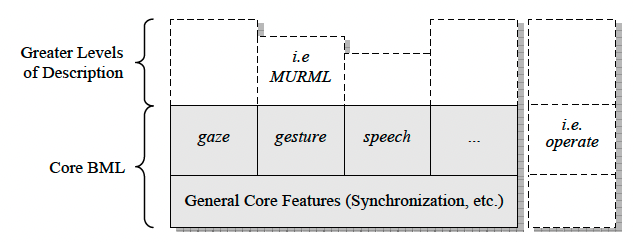
\includegraphics[width=\textwidth]{figures/bml.png}
\captionof{figure}{Extracted from \parencite{vilhjalmsson2007behavior} section 2, BML specification}

This approach aims to maintain the core BML specification entirely agnostic to animation engines, ensuring its independence while striking a judicious equilibrium between expressive detailing and streamlined efficiency. These additional levels provide an avenue for more nuanced or engine-specific depictions of behaviors already outlined in the core BML. This approach fosters flexibility and adaptability, enabling a richer and more detailed representation of behaviors without compromising the core specifications of BML \parencite{vilhjalmsson2007behavior}.




\section{Utterance syntesis}


\subsection{Sign inflections}

In sign language, the utterance synthesis process involves adapting sure signs' forms to reflect their context, known as sign inflection. There are two primary types of inflections. The first is due to sign language's illustrative or iconic nature, where gestures can resemble their meaning or function. The second type involves spatial referencing, which employs physical space to convey relational or locational information. Both inflections are critical for getting accurate and nuanced meanings in sign language \parencite{naert2020survey}.

\subsubsection{Iconic mechanisms}

Iconicity, defined as the presence of non-arbitrary connections between a language's form and meaning, is a distinctive feature of languages, particularly sign languages. Unlike spoken languages, where the relationship between sound and meaning is often arbitrary, sign languages exhibit a higher prevalence of iconicity. In sign languages, many signs bear a visible, intuitive connection to their intentions, making them more directly representational or illustrative of the concepts they convey. This aspect of sign languages highlights a unique dimension in which form and meaning are closely intertwined, offering insights into how different language modalities can structure communication \parencite{iconicityperlman}.

\textcite{naert2020survey} considered size and shape specifiers, classifiers, and role shifts as iconic mechanisms. 

\subsubsection{Spatial referencing}

\textcite{naert2020survey} presented two spatial referencing inflections, such as indicating verbs (see chap 2 section ) and pointing gestures, where pointing gestures involve using the hand, typically the tip of the index finger, to indicate a specific entity or location. These gestures serve multiple purposes: they can identify the subjects or objects of an action, such as in indications of 'I,' 'you,' or 'this one.'

\subsection{Concatenative}

Concatenative synthesis involves the sequential or simultaneous concatenation of pre-recorded or pre-synthesized motion segments across different Sign Language (SL) channels. Transitioning between these motion segments is achieved through motion interpolation or blending techniques. 
Motion blending specifically entails, at each frame, interpolating motions from the database to generate a new motion that preserves the characteristics of the initial motions. The foundation of motion synthesis lies in an annotated database of signs or more detailed motions, from which the system queries to compose the desired utterance. The quality of annotation plays a critical role; the annotation's granularity limits the synthesis's granularity, and the accuracy of data segmentation influences the presence or absence of artifacts in the final animation. The database, created and annotated offline, serves as the primary resource, while the concatenation of signs can be performed in real-time. This approach is particularly well-suited for utterance representations based on sequences of glosses. 

Some approaches use concatenative synthesis for utterance synthesis, such as Hand-Crafted Animations, Automatically Generated Signs, and MoCap Data.


Some research works that follow this approach are the avatars presented in \parencite{braffort2007demonstrations} and \parencite{paulaAvatar} 


\subsection{Articulatory Synthesis}

An alternative method for constructing sign language utterances involves generating them dynamically based on an utterance specification rather than relying on a predetermined database of static motion segments. This approach allows for the inclusion of iconicity, proforms, transitions between signs, and co-occurring phenomena directly within the sign description, enabling a more context-sensitive expression. According to \parencite{naert2020survey} only the GessyCA system \parencite{lebourque1999high} uses the articulatory synthesis alone to build utterances.
Constructing sentences in this manner offers precise control, but providing an utterance description using a sign or gesture specification (as the input for such a system) can be excessively laborious. Additionally, the resulting animation may lack realism and face potential rejection from the Deaf community \parencite{naert2020survey}.

Procedural methods for animating avatars based on sign representations are frequently employed, yet their extension to the utterance level is infrequently observed \parencite{naert2020survey}.


\subsection{Hybrid synthesis}

Hybrid models take advantage of the strengths of concatenative and articulatory synthesis. DePaul University research group implemented this idea on the avatar Paula \parencite{heloir2010real}, their avatar animated with hand-crafted keyframes \parencite{naert2020survey}.


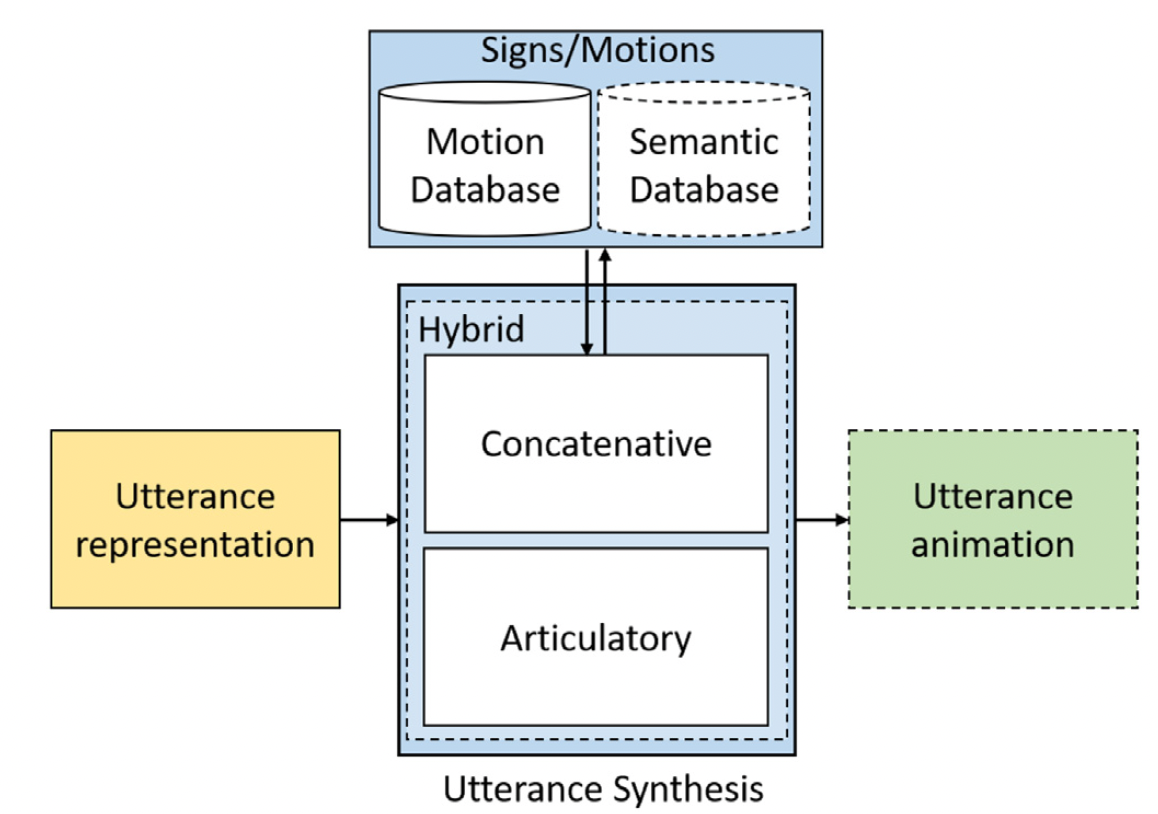
\includegraphics[width=\textwidth]{figures/utterancesynthesis.png}
\captionof{figure}{Extracted from \parencite{naert2020survey} section 5.2, utterance synthesis techniques }

